\chapter{Detailed Evaluation Pipeline Implementation}

This appendix collects the implementation-level artefacts that support the evaluation methodology summarized in Chapter 5. It includes prompt templates, intermediate data formats, algorithm illustrations, and supporting benchmark tables that were moved out of the main chapter to keep the final report concise.

\section{Dataset Generation Artefacts}
The evaluation dataset was constructed by grouping raw SRT transcript segments into larger context windows and prompting an LLM to generate grounded question-answer pairs from each window.

\begin{figure}[H]
  \centering
  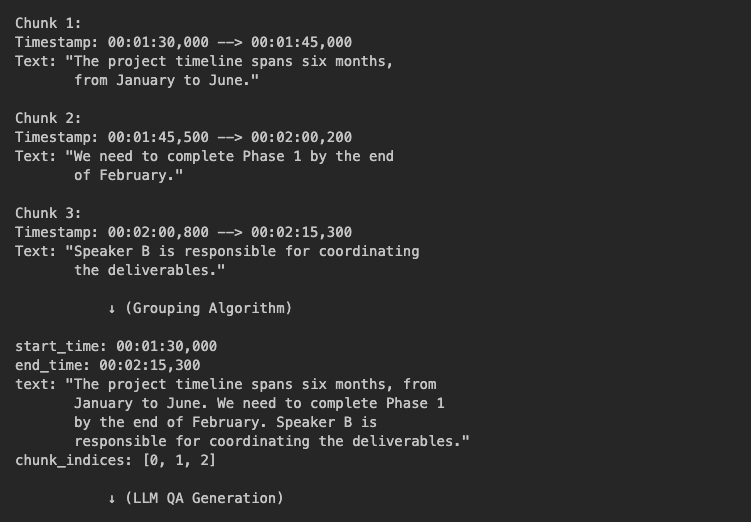
\includegraphics[width=1.0\textwidth]{figures/example_transformation_from_raw_srt_transcript_chunks_to_a_grouped_win.png}
  \caption{Example transformation from raw SRT transcript chunks to a grouped window with temporal metadata}
  \label{fig:fig64}
\end{figure}

\begin{figure}[H]
  \centering
  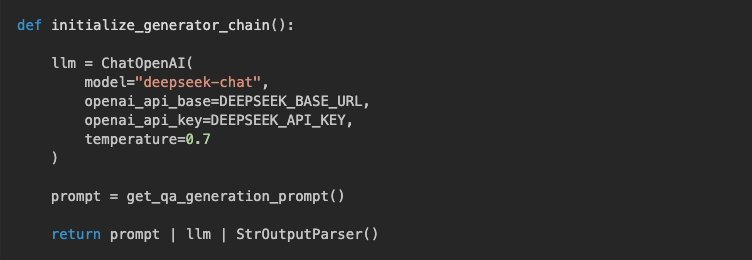
\includegraphics[width=1.0\textwidth]{figures/langchain_pipe_syntax_for_qa_generation_chain.png}
  \caption{LangChain pipe syntax for QA generation chain}
  \label{fig:fig68}
\end{figure}

\begin{figure}[H]
  \centering
  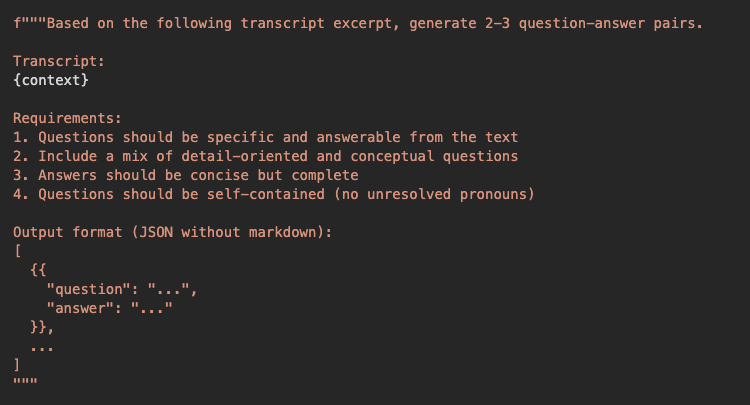
\includegraphics[width=1.0\textwidth]{figures/qa_generation_prompt_template_with_requirements_and_format.png}
  \caption{QA generation prompt template with requirements and format}
  \label{fig:fig48}
\end{figure}

The prompt enforces self-contained questions, grounded answers, and valid JSON output. In practice, generating two to three QA pairs per context window provided a useful balance between dataset size and answer quality.

\begin{figure}[H]
  \centering
  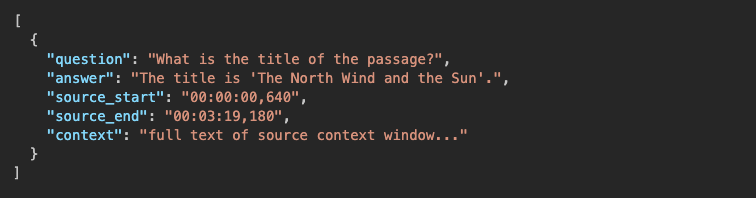
\includegraphics[width=1.0\textwidth]{figures/ground_truth_json_format_example_with_timestamps.png}
  \caption{Ground truth JSON format example with timestamps}
  \label{fig:fig49}
\end{figure}

\begin{table}[H]
  \centering
  \begin{tabular}{|c|c|c|}
    \hline
    \textbf{Field} & \textbf{Type} & \textbf{Description} \\
    \hline
    question & string & Self-contained question derived from context \\
    \hline
    answer & string & Ground truth answer from source text \\
    \hline
    source\_start & string & Start timestamp in SRT format (HH:MM:SS,mmm) \\
    \hline
    source\_end & string & End timestamp in SRT format \\
    \hline
    context & string & Full context window text used for generation \\
    \hline
  \end{tabular}
  \caption{Ground truth schema field descriptions}
  \label{tab:ground-truth-schema}
\end{table}

\section{Metric Implementation Details}
Retrieval relevance was determined by checking whether a retrieved chunk overlapped the ground-truth timestamp range associated with each QA pair.

\begin{figure}[H]
  \centering
  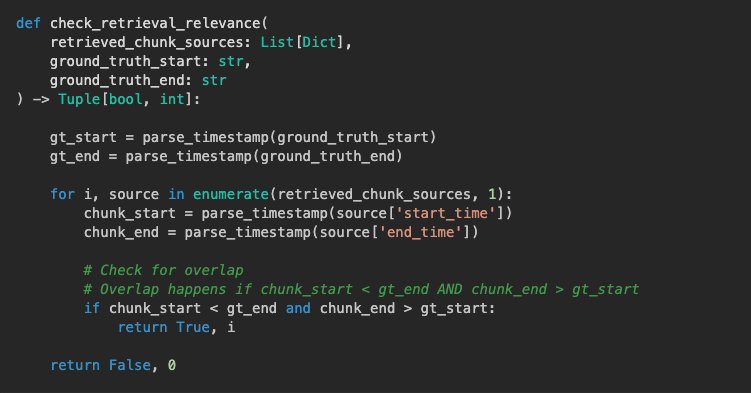
\includegraphics[width=1.0\textwidth]{figures/interval_intersection_algorithm_for_retrieval_relevance_checking.png}
  \caption{Interval intersection algorithm for retrieval relevance checking}
  \label{fig:fig73}
\end{figure}

The same overlap logic supports both Hit Rate and MRR computation by determining whether a relevant chunk exists and, if so, the rank of the first relevant result.

\begin{figure}[H]
  \centering
  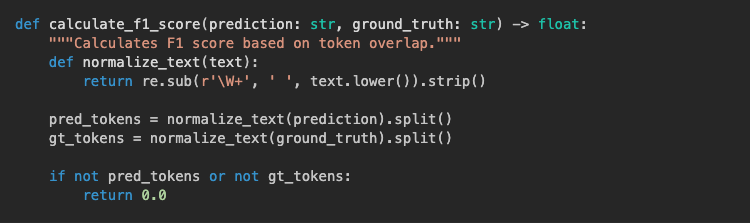
\includegraphics[width=1.0\textwidth]{figures/text_preprocessing_for_token_level_comparison.png}
  \caption{Text preprocessing for token-level comparison}
  \label{fig:fig76}
\end{figure}

\begin{figure}[H]
  \centering
  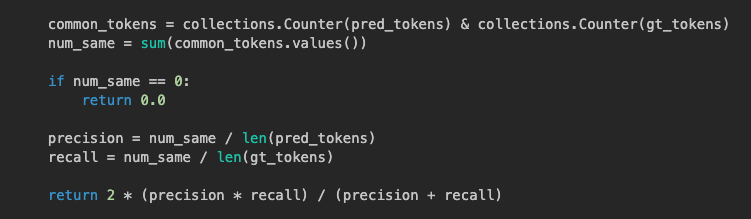
\includegraphics[width=1.0\textwidth]{figures/precision_recall_and_harmonic_mean_calculation_with_counter_intersecti.png}
  \caption{Precision, recall, and harmonic mean calculation with Counter intersection}
  \label{fig:fig77}
\end{figure}

For lexical evaluation, both the prediction and reference answer were normalized before token-level comparison. This reduces the impact of punctuation and formatting differences while preserving word-level content.

\begin{figure}[H]
  \centering
  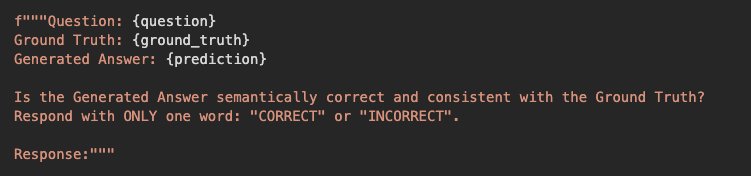
\includegraphics[width=1.0\textwidth]{figures/llm_judge_prompt_template_for_semantic_correctness_evaluation.png}
  \caption{LLM judge prompt template for semantic correctness evaluation}
  \label{fig:fig54}
\end{figure}

The semantic judge receives the question, reference answer, and generated prediction, and returns a binary correctness decision that is then parsed into the final accuracy metric.

\section{Speed Benchmarking Artefacts}
The speed evaluation pipeline was separated from the main quality evaluation loop and executed in an interleaved pattern to reduce prompt-caching bias.

\begin{figure}[H]
  \centering
  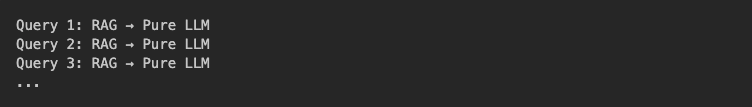
\includegraphics[width=1.0\textwidth]{figures/interleaved_execution_pattern_for_unbiased_speed_benchmarking.png}
  \caption{Interleaved execution pattern for unbiased speed benchmarking}
  \label{fig:fig60}
\end{figure}

\begin{table}[H]
  \centering
  \begin{tabular}{|l|l|}
    \hline
    \textbf{Metric} & \textbf{Description} \\
    \hline
    Mean & Average query time across all timed queries \\
    \hline
    Median & Middle value (robust to outliers) \\
    \hline
    Min & Best-case performance (fastest query) \\
    \hline
    Max & Worst-case performance (slowest query) \\
    \hline
    Std Dev & Standard deviation (consistency measure) \\
    \hline
  \end{tabular}
  \caption{Statistical metrics table for latency analysis}
  \label{tab:latency-statistics}
\end{table}

\begin{table}[H]
  \centering
  \begin{tabular}{|l|>{\raggedright\arraybackslash}p{0.32\textwidth}|>{\raggedright\arraybackslash}p{0.45\textwidth}|}
    \hline
    \textbf{Metric} & \textbf{Formula} & \textbf{Interpretation} \\
    \hline
    Speedup Factor & Pure LLM Mean / RAG Mean & >1: RAG faster, <1: Pure LLM faster, =1: equivalent \\
    \hline
    Time Difference (s) & Pure LLM Mean - RAG Mean & Absolute time saved per query \\
    \hline
    Percentage Faster & (Difference / Pure LLM Mean) $\times$ 100 & Relative improvement percentage \\
    \hline
  \end{tabular}
  \caption{Comparative metrics between RAG and Pure LLM approaches}
  \label{tab:comparative-metrics}
\end{table}
